\section{Softwarearchitektur und Design}

\begin{concept}{Grundlagen und Überblick}
\begin{itemize}
    \item \textbf{Business Analyse:}
    \begin{itemize}
        \item Domänenmodell und Kontextdiagramm
        \item Requirements (funktional und nicht-funktional)
        \item Vision und Stakeholder
    \end{itemize}
    
    \item \textbf{Architektur:}
    \begin{itemize}
        \item Logische Struktur des Systems
        \item Technische Konzeption
        \item Qualitätsanforderungen
    \end{itemize}
    
    \item \textbf{Entwicklung:}
    \begin{itemize}
        \item Use Case / User Story Realisierung
        \item Design-Klassendiagramm (DCD)
        \item Implementierung und Tests
    \end{itemize}
\end{itemize}
Architektur und Design sind eng verzahnt und bauen aufeinander auf:
\begin{itemize}
    \item Architektur definiert das "große Ganze"
    \item Design spezifiziert die Details der Umsetzung
    \item Beides basiert auf Requirements und führt zur Implementation
\end{itemize}
%todo: better resolution image
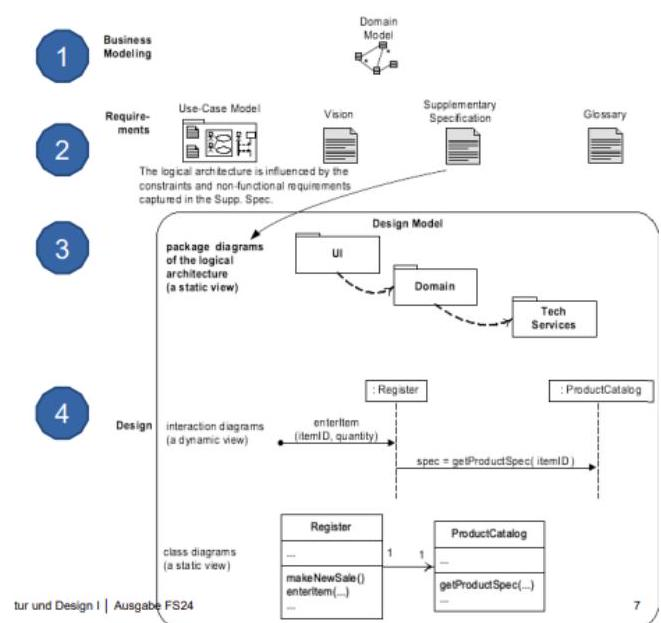
\includegraphics[width=\linewidth]{images/2024_12_29_0d1d7b5551ea1b4b41bdg-07(2)}
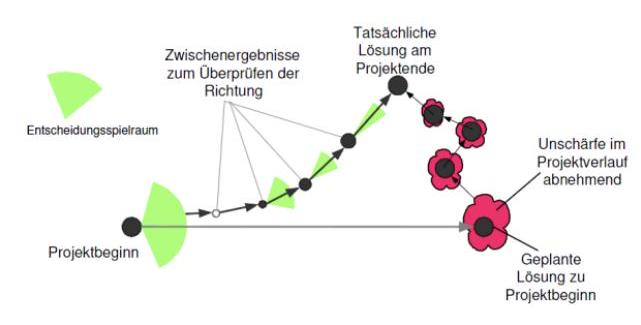
\includegraphics[width=\linewidth]{images/2024_12_29_0d1d7b5551ea1b4b41bdg-08(1)}
\end{concept}

\begin{definition}{Softwarearchitektur}
Die Architektur eines Softwaresystems definiert:

\begin{itemize}
    \item \textbf{Grundlegende Entscheidungen:}
    \begin{itemize}
        \item Programmiersprachen und Plattformen
        \item Aufteilung in Teilsysteme und Komponenten
        \item Schnittstellen zwischen Komponenten
    \end{itemize}
    
    \item \textbf{Strukturelle Aspekte:}
    \begin{itemize}
        \item Verantwortlichkeiten der Teilsysteme
        \item Abhängigkeiten zwischen Komponenten
        \item Einsatz von Basis-Technologien/Frameworks
    \end{itemize}
    
    \item \textbf{Qualitätsaspekte:}
    \begin{itemize}
        \item Erfüllung nicht-funktionaler Anforderungen
        \item Maßnahmen für Performance, Skalierbarkeit etc.
        \item Fehlertoleranz und Ausfallsicherheit
    \end{itemize}
\end{itemize}
\end{definition}

\begin{concept}{Architekturanalyse}\\
erfolgt iterativ mit den Anforderungen (Twin Peaks Model):

\begin{itemize}
    \item \textbf{Anforderungsanalyse:}
    \begin{itemize}
        \item Analyse funktionaler und nicht-funktionaler Anforderungen
        \item Prüfung der Qualität und Stabilität der Anforderungen
        \item Identifikation von Lücken und impliziten Anforderungen
    \end{itemize}
    
    \item \textbf{Architekturentscheidungen:}
    \begin{itemize}
        \item Abstimmung mit Stakeholdern
        \item Berücksichtigung von Randbedingungen
        \item Vorausschauende Planung für zukünftige Änderungen
    \end{itemize}
\end{itemize}

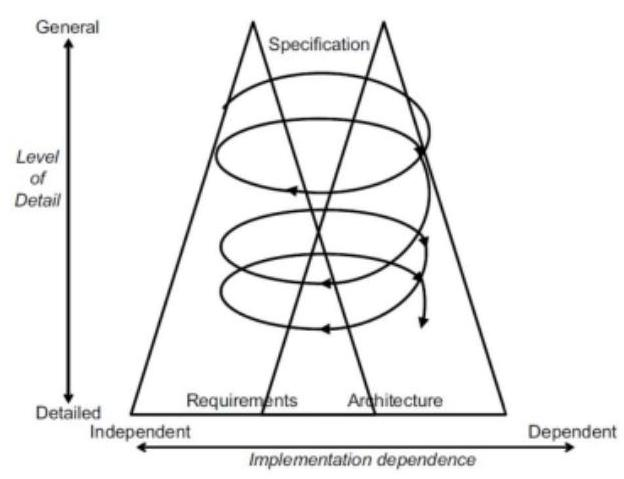
\includegraphics[width=0.9\linewidth]{images/2024_12_29_0d1d7b5551ea1b4b41bdg-08}
\end{concept}

\begin{theorem}{Qualitätsanforderungen}\\
\textbf{ISO 25010:}
\begin{itemize}
    \item Hierarchische Struktur für nicht-funktionale Anforderungen
    \item Definierte Hauptcharakteristiken und Subcharakteristiken
    \item Messbare Metriken für jede Anforderung
    \item Ermöglicht präzise Formulierung und Verifikation
\end{itemize}

\textbf{FURPS+:}
\begin{itemize}
    \item \textbf{F}unctionality (Funktionalität)
    \item \textbf{U}sability (Benutzerfreundlichkeit)
    \item \textbf{R}eliability (Zuverlässigkeit)
    \item \textbf{P}erformance (Leistung)
    \item \textbf{S}upportability (Wartbarkeit)
    \item \textbf{+}: Implementation, Interface, Operations, Packaging, Legal
\end{itemize}
\end{theorem}

\begin{KR}{Architekturanalyse durchführen}\\
\textbf{1. Anforderungen analysieren}
\begin{itemize}
    \item Funktionale Anforderungen gruppieren
    \item Nicht-funktionale Anforderungen priorisieren
    \item Randbedingungen identifizieren
\end{itemize}

\textbf{2. Qualitätsziele definieren}
\begin{itemize}
    \item Messbare Kriterien festlegen
    \item Priorisierung vornehmen
    \item Trade-offs identifizieren
\end{itemize}

\textbf{3. Architekturentscheidungen treffen}
\begin{itemize}
    \item Alternativen evaluieren
    \item Entscheidungen dokumentieren
    \item Mit Stakeholdern abstimmen
\end{itemize}

\textbf{4. Validierung durchführen}
\begin{itemize}
    \item Architektur-Reviews planen
    \item Prototypen erstellen
    \item Risiken bewerten
\end{itemize}
\end{KR}

\pagebreak

\subsection{Architektur-Design}

\begin{concept}{Modulkonzept}\\
Ein Modul (Baustein, Komponente) wird charakterisiert durch:

\begin{itemize}
    \item \textbf{Eigenschaften:}
    \begin{itemize}
        \item Autarkes Teilsystem (geringe externe Abhängigkeiten)
        \item Klar definierte Schnittstellen nach außen
        \item Enthält alle benötigten Funktionen und Daten
        \item Kann als Paket, Library, Komponente oder Service realisiert werden
    \end{itemize}
    
    \item \textbf{Bewertungskriterien:}
    \begin{itemize}
        \item \textbf{Kohäsion:} Stärke des inneren Zusammenhangs
        \item \textbf{Kopplung:} Grad der Abhängigkeit zu anderen Modulen
    \end{itemize}
\end{itemize}
\end{concept}

\begin{definition}{Schnittstellen}\\
Module kommunizieren über definierte Schnittstellen:

\begin{itemize}
    \item \textbf{Exportierte Schnittstellen:}
    \begin{itemize}
        \item Definieren angebotene Funktionalität
        \item Vertraglich garantierte Leistungen
        \item Einzige nach außen sichtbare Information
    \end{itemize}
    
    \item \textbf{Importierte Schnittstellen:}
    \begin{itemize}
        \item Von anderen Modulen benötigte Funktionalität
        \item Definieren Abhängigkeiten
        \item Sollten minimiert werden (Low Coupling)
    \end{itemize}
\end{itemize}
\end{definition}

\begin{concept}{Architektursichten (4+1 View Model)}\\
Verschiedene Perspektiven auf die Architektur:

\begin{itemize}
    \item \textbf{Logical View:}
    \begin{itemize}
        \item Funktionalität des Systems
        \item Schichten, Subsysteme, Pakete
        \item Klassen und Schnittstellen
    \end{itemize}
    
    \item \textbf{Process View:}
    \begin{itemize}
        \item Laufzeitverhalten
        \item Prozesse und Threads
        \item Performance und Skalierung
    \end{itemize}
    
    \item \textbf{Development View:}
    \begin{itemize}
        \item Implementierungsstruktur
        \item Quellcode-Organisation
        \item Build und Deployment
    \end{itemize}
    
    \item \textbf{Physical View:}
    \begin{itemize}
        \item Hardware-Topologie
        \item Verteilung der Software
        \item Netzwerkkommunikation
    \end{itemize}
    
    \item \textbf{+1: Scenarios:}
    \begin{itemize}
        \item Wichtige Use Cases
        \item Validierung der Architektur
        \item Integration der anderen Views
    \end{itemize}
\end{itemize}

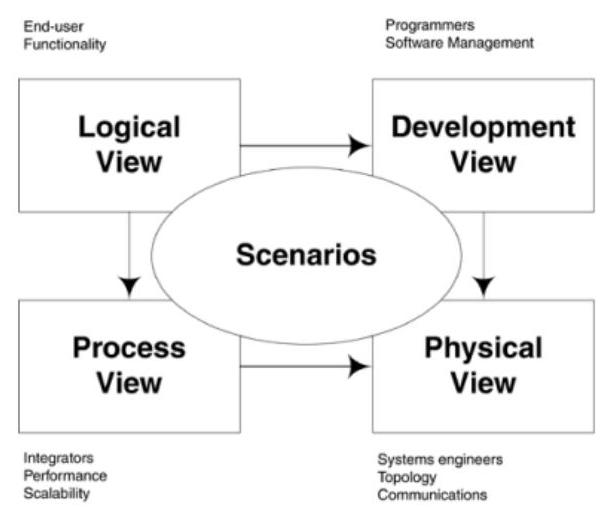
\includegraphics[width=0.9\linewidth]{images/2024_12_29_0d1d7b5551ea1b4b41bdg-09}
\end{concept}

\begin{theorem}{Qualitaetskriterien und deren Umsetzung}\\
Strategien zur Erfüllung von Qualitätsanforderungen:

\textbf{Performance:}
\begin{itemize}
    \item Resource Pooling (Wiederverwendung von Ressourcen)
    \item Caching (Zwischenspeicherung)
    \item Parallelisierung (Verteilung der Last)
    \item Lazy Loading (Verzögerte Initialisierung)
\end{itemize}

\textbf{Skalierbarkeit:}
\begin{itemize}
    \item Horizontale Skalierung (mehr Instanzen)
    \item Vertikale Skalierung (mehr Ressourcen)
    \item Load Balancing (Lastverteilung)
    \item Partitionierung (Datenaufteilung)
\end{itemize}

\textbf{Wartbarkeit:}
\begin{itemize}
    \item Separation of Concerns (Trennung der Zuständigkeiten)
    \item Information Hiding (Kapselung)
    \item Standardisierung (einheitliche Patterns)
    \item Modularisierung (unabhängige Komponenten)
\end{itemize}

\textbf{Zuverlässigkeit:}
\begin{itemize}
    \item Redundanz (Mehrfachsysteme)
    \item Fehlertoleranz (Graceful Degradation)
    \item Monitoring (Überwachung)
    \item Backup und Recovery
\end{itemize}
\end{theorem}

\begin{KR}{Best Practices im Architekturentwurf}\\
\textbf{1. Analyse und Planung}
\begin{itemize}
    \item Anforderungen priorisieren
    \item Qualitätsziele definieren
    \item Constraints identifizieren
    \item Stakeholder einbinden
\end{itemize}

\textbf{2. Design-Prinzipien}
\begin{itemize}
    \item Separation of Concerns
    \item Single Responsibility
    \item Information Hiding
    \item Don't Repeat Yourself (DRY)
\end{itemize}

\textbf{3. Strukturierung}
\begin{itemize}
    \item Klare Schichtenarchitektur
    \item Definierte Schnittstellen
    \item Lose Kopplung
    \item Hohe Kohäsion
\end{itemize}

\textbf{4. Dokumentation}
\begin{itemize}
    \item Architekturentscheidungen
    \item Begründungen
    \item Alternativen
    \item Trade-offs
\end{itemize}
\end{KR}

\subsection{Architekturmuster}

\begin{concept}{Übersicht Architekturmuster}\\
Grundlegende Architekturmuster für Software-Systeme:

\begin{itemize}
    \item \textbf{Layered Pattern:} 
    \begin{itemize}
        \item Strukturierung in horizontale Schichten
        \item Klare Trennung der Verantwortlichkeiten
        \item Abhängigkeiten nur nach unten
    \end{itemize}
    
    \item \textbf{Client-Server Pattern:}
    \begin{itemize}
        \item Verteilung von Diensten
        \item Zentralisierte Ressourcen
        \item Mehrere Clients pro Server
    \end{itemize}
    
    \item \textbf{Master-Slave Pattern:}
    \begin{itemize}
        \item Verteilung von Aufgaben
        \item Zentrale Koordination
        \item Parallelverarbeitung
    \end{itemize}
    
    \item \textbf{Pipe-Filter Pattern:}
    \begin{itemize}
        \item Datenstromverarbeitung
        \item Verkettung von Operationen
        \item Wiederverwendbare Filter
    \end{itemize}
    
    \item \textbf{Broker Pattern:}
    \begin{itemize}
        \item Vermittlung zwischen Komponenten
        \item Entkopplung von Diensten
        \item Zentrale Koordination
    \end{itemize}
    
    \item \textbf{Event-Bus Pattern:}
    \begin{itemize}
        \item Asynchrone Kommunikation
        \item Publisher-Subscriber Modell
        \item Lose Kopplung
    \end{itemize}
\end{itemize}
\end{concept}

\begin{concept}{Schichtenarchitektur (Layered Architecture)}\\
Organisation des Systems in hierarchische Schichten:

\textbf{Typische Schichten:}
\begin{itemize}
    \item Präsentationsschicht (UI)
    \item Anwendungsschicht (Application Logic)
    \item Geschäftslogikschicht (Domain Logic)
    \item Datenzugriffsschicht (Data Access)
\end{itemize}

\textbf{Prinzipien:}
\begin{itemize}
    \item Schichten kommunizieren nur mit direkten Nachbarn
    \item Abhängigkeiten nur nach unten
    \item Jede Schicht kapselt ihre Implementierung
    \item Höhere Schichten sind von unteren abhängig
\end{itemize}

\begin{lstlisting}[language=Java, style=basesmol]
// Praesentationsschicht
public class CustomerController {
    private CustomerService service;
    
    public CustomerDTO getCustomer(String id) {
        return service.findCustomer(id);
    }
}

// Anwendungsschicht
public class CustomerService {
    private CustomerRepository repository;
    
    public CustomerDTO findCustomer(String id) {
        Customer customer = repository.findById(id);
        return CustomerDTO.from(customer);
    }
}

// Geschaeftslogikschicht
public class Customer {
    private CustomerId id;
    private String name;
    
    public void updateName(String newName) {
        validateName(newName);
        this.name = newName;
    }
}

// Datenzugriffsschicht
public class CustomerRepository {
    public Customer findById(String id) {
        // Datenbankzugriff
    }
}
\end{lstlisting}
\end{concept}

\begin{concept}{Clean Architecture}\\
Architektur-Prinzipien nach Robert C. Martin:

\textbf{Hauptprinzipien:}
\begin{itemize}
    \item Unabhängigkeit von Frameworks
    \item Unabhängigkeit von UI
    \item Unabhängigkeit von Datenbank
    \item Testbarkeit ohne externe Systeme
\end{itemize}

\textbf{Schichten (von innen nach außen):}
\begin{itemize}
    \item \textbf{Entities:} 
    \begin{itemize}
        \item Zentrale Geschäftsregeln
        \item Unternehmensweit gültig
        \item Höchste Stabilität
    \end{itemize}
    
    \item \textbf{Use Cases:}
    \begin{itemize}
        \item Anwendungsspezifische Geschäftsregeln
        \item Orchestrierung der Entities
        \item Anwendungslogik
    \end{itemize}
    
    \item \textbf{Interface Adapters:}
    \begin{itemize}
        \item Konvertierung von Daten
        \item Präsentation und Controller
        \item Gateway-Implementierungen
    \end{itemize}
    
    \item \textbf{Frameworks \& Drivers:}
    \begin{itemize}
        \item UI-Framework
        \item Datenbank
        \item Externe Schnittstellen
    \end{itemize}
\end{itemize}

\begin{lstlisting}[language=Java, style=basesmol]
// Entity (innerste Schicht)
public class Customer {
    private CustomerId id;
    private String name;
    
    public void validateName(String name) {
        // Domaenenregeln fuer Namen
    }
}

// Use Case (Business Rules)
public class RegisterCustomerUseCase {
    public void execute(RegisterCustomerCommand cmd) {
        Customer customer = new Customer(cmd.getName());
        customer.validateName(cmd.getName());
        repository.save(customer);
    }
}

// Interface Adapter
public class CustomerController {
    private RegisterCustomerUseCase useCase;
    
    public ResponseEntity<CustomerDTO> register(
            CustomerRequest request) {
        useCase.execute(
            new RegisterCustomerCommand(request.getName())
        );
        return ResponseEntity.ok().build();
    }
}
\end{lstlisting}
\end{concept}

\begin{concept}{Microservices Architektur}\\
Verteilte Architektur mit unabhängigen Services:

\textbf{Charakteristiken:}
\begin{itemize}
    \item Unabhängig entwickelbar und deploybar
    \item Eigene Datenhaltung pro Service
    \item Lose Kopplung
    \item API-basierte Kommunikation
\end{itemize}

\textbf{Patterns:}
\begin{itemize}
    \item Service Discovery
    \item API Gateway
    \item Circuit Breaker
    \item Event Sourcing
    \item CQRS (Command Query Responsibility Segregation)
\end{itemize}

\begin{lstlisting}[language=Java, style=basesmol]
@Service
public class OrderService {
    private final CustomerClient customerClient;
    private final PaymentClient paymentClient;
    
    @CircuitBreaker(name = "order")
    public OrderResult createOrder(OrderRequest request) {
        // Kundeninformationen laden
        CustomerInfo customer = 
            customerClient.getCustomer(request.getCustomerId());
            
        // Zahlungsabwicklung
        PaymentResult payment = 
            paymentClient.processPayment(request.getAmount());
            
        // Order erstellen
        return createOrderWithPayment(customer, payment);
    }
}
\end{lstlisting}
\end{concept}

\begin{concept}{Event-Driven Architecture (EDA)}\\
Architekturstil basierend auf der Erzeugung, Erkennung und Verarbeitung von Events:

\textbf{Kernkomponenten:}
\begin{itemize}
    \item \textbf{Event Producer:} Erzeugt Events
    \item \textbf{Event Channel:} Transportiert Events
    \item \textbf{Event Consumer:} Verarbeitet Events
    \item \textbf{Event Processor:} Transformiert Events
\end{itemize}

\begin{lstlisting}[language=Java, style=basesmol]
// Event Definition
public class OrderCreatedEvent {
    private final OrderId orderId;
    private final CustomerId customerId;
    private final Money totalAmount;
    private final LocalDateTime timestamp;
}

// Event Producer
@Service
public class OrderService {
    private final EventPublisher eventPublisher;
    
    public Order createOrder(OrderRequest request) {
        Order order = orderRepository.save(
            new Order(request));
        
        eventPublisher.publish(new OrderCreatedEvent(
            order.getId(),
            order.getCustomerId(),
            order.getTotalAmount(),
            LocalDateTime.now()
        ));
        
        return order;
    }
}

// Event Consumer
@Service
public class NotificationService {
    @EventListener
    public void handleOrderCreated(
            OrderCreatedEvent event) {
        sendConfirmationEmail(event.getCustomerId());
    }
}
\end{lstlisting}
\end{concept}

\begin{concept}{Integration Patterns}\\
Muster für die Integration verschiedener Systeme:

\textbf{Hauptkategorien:}
\begin{itemize}
    \item \textbf{File Transfer:}
    \begin{itemize}
        \item Datenaustausch über Dateien
        \item Batch-Verarbeitung
        \item Einfache Integration
    \end{itemize}
    
    \item \textbf{Shared Database:}
    \begin{itemize}
        \item Gemeinsame Datenbasis
        \item Direkte Integration
        \item Hohe Kopplung
    \end{itemize}
    
    \item \textbf{Remote Procedure Call:}
    \begin{itemize}
        \item Synchrone Kommunikation
        \item Direkter Methodenaufruf
        \item Service-Orientierung
    \end{itemize}
    
    \item \textbf{Messaging:}
    \begin{itemize}
        \item Asynchrone Kommunikation
        \item Message Broker
        \item Lose Kopplung
    \end{itemize}
\end{itemize}

\textbf{Spezifische Patterns:}
\begin{itemize}
    \item Message Router
    \item Message Translator
    \item Message Filter
    \item Content Enricher
    \item Message Store
\end{itemize}
\end{concept}

\subsection{Objektorientiertes Design}

\begin{concept}{GRASP Prinzipien}\\
General Responsibility Assignment Software Patterns - Grundlegende Prinzipien für die Zuweisung von Verantwortlichkeiten:

\textbf{Information Expert:}
\begin{itemize}
    \item Zuständigkeit basierend auf Information
    \item Klasse mit relevanten Daten übernimmt Aufgabe
    \item Fördert Kapselung und Kohäsion
\end{itemize}

\textbf{Creator:}
\begin{itemize}
    \item Verantwortung für Objekterstellung
    \item Basierend auf Beziehungen (enthält, aggregiert)
    \item Starke Verwendungsbeziehung
\end{itemize}

\textbf{Controller:}
\begin{itemize}
    \item Koordination von Systemoperationen
    \item Erste Anlaufstelle nach UI
    \item Fassade für Subsystem
\end{itemize}

\textbf{Low Coupling:}
\begin{itemize}
    \item Minimale Abhängigkeiten
    \item Erhöht Wiederverwendbarkeit
    \item Erleichtert Änderungen
\end{itemize}

\textbf{High Cohesion:}
\begin{itemize}
    \item Fokussierte Verantwortlichkeiten
    \item Zusammengehörige Funktionalität
    \item Wartbare Klassen
\end{itemize}

\begin{lstlisting}[language=Java, style=basesmol]
// Information Expert
public class Order {
    private List<OrderLine> lines;
    
    // Order kennt seine eigenen Daten
    public Money calculateTotal() {
        return lines.stream()
                   .map(OrderLine::getSubTotal)
                   .reduce(Money.ZERO, Money::add);
    }
}

// Creator
public class Order {
    // Order erstellt OrderLines 
    // (enthaelt und verwendet sie)
    public void addProduct(Product product, int quantity) {
        lines.add(new OrderLine(product, quantity));
    }
}

// Controller
public class OrderController {
    private OrderService orderService;
    
    // Koordiniert Systemoperationen
    public OrderResponse createOrder(OrderRequest request) {
        Order order = orderService.createOrder(request);
        return OrderResponse.from(order);
    }
}
\end{lstlisting}
\end{concept}

\begin{concept}{Responsibility Driven Design}\\
Designansatz basierend auf Verantwortlichkeiten und Kollaborationen:

\textbf{Verantwortlichkeiten:}
\begin{itemize}
    \item \textbf{Doing:}
    \begin{itemize}
        \item Aktionen ausführen
        \item Berechnungen durchführen
        \item Andere Objekte steuern
    \end{itemize}
    
    \item \textbf{Knowing:}
    \begin{itemize}
        \item Eigene Daten kennen
        \item Verwandte Objekte kennen
        \item Berechnete Informationen
    \end{itemize}
\end{itemize}

\textbf{Kollaborationen:}
\begin{itemize}
    \item Klare Rollen definieren
    \item Aufgaben verteilen
    \item Interfaces abstimmen
\end{itemize}
\end{concept}

\subsection{UML-Modellierung}

\begin{concept}{Grundlagen der UML-Modellierung}\\
UML (Unified Modeling Language) wird im Design auf zwei Arten verwendet:

\textbf{Statische Modelle:}
\begin{itemize}
    \item Struktur des Systems
    \item Klassendiagramme, Paketdiagramme
    \item Fokus auf Pakete, Klassen, Attribute
    \item Keine Methodenimplementierung
\end{itemize}

\textbf{Dynamische Modelle:}
\begin{itemize}
    \item Verhalten des Systems
    \item Sequenz-, Zustands-, Aktivitätsdiagramme
    \item Fokus auf Logik und Verhalten
    \item Methodenimplementierung
\end{itemize}
\end{concept}

\begin{concept}{UML Diagrammtypen}\\
\textbf{Klassendiagramm:}
\begin{itemize}
    \item Klassen mit Attributen und Methoden
    \item Beziehungen zwischen Klassen
    \item Vererbung und Implementierung
    \item Multiplizitäten und Rollen
\end{itemize}

\textbf{Sequenzdiagramm:}
\begin{itemize}
    \item Zeitlicher Ablauf von Interaktionen
    \item Nachrichtenaustausch zwischen Objekten
    \item Synchrone und asynchrone Kommunikation
    \item Alternative Abläufe und Schleifen
\end{itemize}

\textbf{Zustandsdiagramm:}
\begin{itemize}
    \item Zustandsübergänge eines Objekts
    \item Events und Guards
    \item Composite States
    \item Entry/Exit Actions
\end{itemize}

\textbf{Aktivitätsdiagramm:}
\begin{itemize}
    \item Ablauf von Geschäftsprozessen
    \item Kontrollfluss und Datenfluss
    \item Parallelität und Synchronisation
    \item Swimlanes für Verantwortlichkeiten
\end{itemize}
\end{concept}

\begin{example2}{UML im Design}\\
\textbf{Klassendiagramm für Order Management:}

\begin{lstlisting}[language=Java, style=basesmol]
public class Order {
    private OrderId id;
    private Customer customer;
    private List<OrderLine> lines;
    private OrderStatus status;
    
    public Money calculateTotal() {
        return lines.stream()
                   .map(OrderLine::getSubTotal)
                   .reduce(Money.ZERO, Money::add);
    }
    
    public void addProduct(Product product, int qty) {
        lines.add(new OrderLine(product, qty));
    }
}

public class OrderLine {
    private Product product;
    private int quantity;
    
    public Money getSubTotal() {
        return product.getPrice()
                     .multiply(quantity);
    }
}

@Service
public class OrderService {
    private OrderRepository repository;
    
    public Order createOrder(OrderRequest request) {
        Order order = new Order(request.getCustomerId());
        request.getItems().forEach(item -> 
            order.addProduct(item.getProduct(), 
                           item.getQuantity()));
        return repository.save(order);
    }
}
\end{lstlisting}
\end{example2}

\begin{example2}{Sequenzdiagramm für Bestellprozess}\\
\textbf{Implementierung einer Bestellverarbeitung:}

\begin{lstlisting}[language=Java, style=basesmol]
@RestController
public class OrderController {
    private final OrderService orderService;
    private final PaymentService paymentService;
    
    public OrderResponse createOrder(
            OrderRequest request) {
        // Validiere Bestellung
        validateOrder(request);
        
        // Erstelle Order
        Order order = orderService.createOrder(request);
        
        // Prozessiere Zahlung
        PaymentResult payment = 
            paymentService.processPayment(
                order.getId(), 
                order.getTotal()
            );
        
        // Update Order Status
        if (payment.isSuccessful()) {
            order.confirm();
            orderService.save(order);
        }
        
        return OrderResponse.from(order);
    }
}
\end{lstlisting}
\end{example2}

\begin{example2}{Zustandsdiagramm für Bestellstatus}\\
\textbf{Implementation des State Patterns:}

\begin{lstlisting}[language=Java, style=basesmol]
public interface OrderState {
    void process(Order order);
    void cancel(Order order);
    void ship(Order order);
}

public class NewOrderState implements OrderState {
    @Override
    public void process(Order order) {
        validateOrder(order);
        order.setState(new ProcessingState());
    }
    
    @Override
    public void cancel(Order order) {
        order.setState(new CancelledState());
    }
    
    @Override
    public void ship(Order order) {
        throw new IllegalStateException(
            "Cannot ship new order");
    }
}

public class Order {
    private OrderState state;
    
    public void process() {
        state.process(this);
    }
    
    void setState(OrderState newState) {
        this.state = newState;
    }
}
\end{lstlisting}
\end{example2}

\begin{KR}{UML Diagrammauswahl}\\
\textbf{Auswahlkriterien:}

\begin{enumerate}
    \item \textbf{Ziel der Modellierung}
    \begin{itemize}
        \item Struktur darstellen -> Klassendiagramm
        \item Abläufe zeigen -> Sequenzdiagramm
        \item Zustände dokumentieren -> Zustandsdiagramm
        \item Prozesse beschreiben -> Aktivitätsdiagramm
    \end{itemize}
    
    \item \textbf{Zielgruppe}
    \begin{itemize}
        \item Entwickler -> detaillierte technische Diagramme
        \item Stakeholder -> vereinfachte Übersichtsdiagramme
        \item Architekten -> Architekturdiagramme
    \end{itemize}
    
    \item \textbf{Detailgrad}
    \begin{itemize}
        \item Überblick -> wenige wichtige Elemente
        \item Detaildesign -> vollständige Details
        \item Implementation -> code-nahe Darstellung
    \end{itemize}
    
    \item \textbf{Phase im Projekt}
    \begin{itemize}
        \item Analyse -> konzeptuelle Modelle
        \item Design -> Designmodelle
        \item Implementation -> detaillierte Modelle
    \end{itemize}
\end{enumerate}
\end{KR}

\begin{example2}{Aktivitätsdiagramm für Geschäftsprozess}\\
\textbf{Implementation eines Workflow:}

\begin{lstlisting}[language=Java, style=basesmol]
public class OrderProcessor {
    public void processOrder(Order order) {
        // Parallel processing
        CompletableFuture.allOf(
            validateInventory(order),
            validatePayment(order)
        ).thenRun(() -> {
            if (order.isValid()) {
                fulfillOrder(order);
            } else {
                handleValidationFailure(order);
            }
        });
    }
    
    private CompletableFuture<Void> validateInventory(
            Order order) {
        return CompletableFuture.runAsync(() -> {
            order.getItems().forEach(item -> {
                if (!inventoryService.isAvailable(item)) {
                    throw new OutOfStockException(item);
                }
            });
        });
    }
}
\end{lstlisting}
\end{example2}